%%%%%%%% ICML 2018 EXAMPLE LATEX SUBMISSION FILE %%%%%%%%%%%%%%%%%

\documentclass{article}

% Recommended, but optional, packages for figures and better typesetting:
\usepackage{microtype}
\usepackage{graphicx}
\usepackage{hyperref}
\usepackage{cleveref}
\usepackage{bm}
\usepackage{amsthm}
\usepackage{amsfonts}
\usepackage{subfigure}
\usepackage{stmaryrd}
\usepackage{booktabs} % for professional tables

% hyperref makes hyperlinks in the resulting PDF.
% If your build breaks (sometimes temporarily if a hyperlink spans a page)
% please comment out the following usepackage line and replace
% \usepackage{icml2018} with \usepackage[nohyperref]{icml2018} above.
\usepackage{amsmath}

% Attempt to make hyperref and algorithmic work together better:
\newcommand{\theHalgorithm}{\arabic{algorithm}}

\newcommand{\norm}[1]{\left\lVert#1\right\rVert}
\newcommand{\abs}[1]{\left|#1\right|}
\newcommand{\diag}[1]{\text{diag}\left(#1\right)}
\newcommand{\intint}[1]{\left\llbracket#1\right\rrbracket}
\newtheorem{proposition}{Proposition}[section]

% Use the following line for the initial blind version submitted for review:
\usepackage{icml2018}

% If accepted, instead use the following line for the camera-ready submission:
%\usepackage[accepted]{icml2018}

% The \icmltitle you define below is probably too long as a header.
% Therefore, a short form for the running title is supplied here:
\icmltitlerunning{Learning Neural Network size with ShrinkNets}

\begin{document}

\twocolumn[
\icmltitle{Learning Network Size while Training with ShrinkNets}

% It is OKAY to include author information, even for blind
% submissions: the style file will automatically remove it for you
% unless you've provided the [accepted] option to the icml2018
% package.

% List of affiliations: The first argument should be a (short)
% identifier you will use later to specify author affiliations
% Academic affiliations should list Department, University, City, Region, Country
% Industry affiliations should list Company, City, Region, Country

% You can specify symbols, otherwise they are numbered in order.
% Ideally, you should not use this facility. Affiliations will be numbered
% in order of appearance and this is the preferred way.
\icmlsetsymbol{equal}{*}

\begin{icmlauthorlist}
\icmlauthor{Guillaume Leclerc}{mit}
\icmlauthor{Raul Castro Fernandez}{mit}
\icmlauthor{Manasi Vartak}{mit}
\icmlauthor{Martin Jaggi}{epfl}
\icmlauthor{Samuel Madden}{mit}
\end{icmlauthorlist}

\icmlaffiliation{mit}{Computer Science and Artificial Intelligence Laboratories, Massachusetts Institute of Technology, Cambridge, Massachusetts, USA}

\icmlaffiliation{epfl}{Swiss Federal Institute of Technology, Lausanne, Switzerland}

\icmlcorrespondingauthor{Guillaume Leclerc}{leclerc@mit.edu}

% You may provide any keywords that you
% find helpful for describing your paper; these are used to populate
% the "keywords" metadata in the PDF but will not be shown in the document
\icmlkeywords{Machine Learning, ICML}

\vskip 0.3in
]

% this must go after the closing bracket ] following \twocolumn[ ...

% This command actually creates the footnote in the first column
% listing the affiliations and the copyright notice.
% The command takes one argument, which is text to display at the start of the footnote.
% The \icmlEqualContribution command is standard text for equal contribution.
% Remove it (just {}) if you do not need this facility.

%\printAffiliationsAndNotice{}  % leave blank if no need to mention equal contribution
\printAffiliationsAndNotice{} % otherwise use the standard text.

\begin{abstract}
  Let's write the abstract at the end
\end{abstract}

\section{Tentative outline}

\begin{itemize}
  \item We want to figure out what is the proper network size
  \item If we had a oversized network and for each neuron we would have an on/off switch, we could optimize the state of each switch to achieve any size/accuracy tradeof (we can prove that, do we care ?)
  \item Solving such problem is NP-Hard
  \item We could approximate the binary switch by relaxing them and doing L1 loss instead of L0 loss
  \item This is the definition of Shrinknets
  \item group sparsity tries to achieve a similar goal but with a different formulation
  \item How are they related ?
  \item If we add a specific constraint on our formulation we obtain the group sparsity one (proven)
  \item We conclude that without this constraint our formulation has more degree of freedom
  \item What happen when we drop this constraint
  \item The problem becomes non-convex and without a global minimum
  \item Not having a global minimum is bad, how can we solve that ?
  \item Adding an extra regularization parameter allow us to have a global minimum (a lot of them actually)
  \item Now we have a framework to switch on and of neurons
  \item We are still doing useless computation for neurons that will stay off forever, if we pruned them then we would speed up training
  \item Define the strategy to detect "forever dead" neurons
  \item (should we talk about the software architecture ?)
  \item now we evaluate the system
  \item First we show that our system has indeed more freedom than Group sparsity by showing that for any given amount of sparsity it can fit closer than the previous method
  \item On the same problem we show that removing neurons on the fly does not dramatically reduce accuracy (we might not be able to see any difference in performance for a linear/logistic regression though)
  \item We show that works with Bigger networks (multi layers perceptrons and CNNs), describe the training dynamics, discuss the shape we obtain
  \item Show that it is easier to do hyper-parameter optimization on the regularization parameter that the size of each layer. I think a nice experiment would be to plot the evolution of the final size of a two layer network (so going from a lambda to two sizes). And plot the trajectory in the "size space" as we decrease lambda. It would show how the system trades off the budget between the two layer in a nice and visual way
  \item Then we evaluate performance
\end{itemize}

\section{Introduction}

\section{ShrinkNets}

\subsection{Motivation}

\subsection{Notations}

\par In order to avoid any potential ambiguity, in this section we will
describe in details the mathematical notations used in this article. Non-bold
letters represent scalar values, while bold lowercase and upper case
repectively denote vectors and matrices. $\bm{A}^T$ stands for the transpose of
the matrix $\bm{A}$. Subscripts are used to index particular elements of
vectors and matrices. $\bm{x}_i$, $\bm{A}_i$, $\left(\bm{A}^T\right)_j$ and
$\bm{A}_{i,j}$ respectively correspond to the $i^{th}$ component of $\bm{x}$,
the $i^{th}$ row of $\bm{A}$, the $j^{th}$ column of $\bm{A}$ and the $j^{th}$
component of the $i^{th}$ row of $\bm{A}$. All the following definitions assume
$\bm{A}$ to be an $n\times p$ matrix.  For any vetor $\bm{b}$ with $n$
components, we define $\diag{\bm{b}}$ a $n\times n$ matrix such that: $\forall
1 \leq i \leq n$, $\diag{\bm{b}}_{i, i} = \bm{b}_i$ and $0$ otherwise.  For any $l \in \left[0, +\infty\right]$ we define the norm: $\norm{\bm{A}}_l =
\left(\sum_{i=1}^n \sum_{j=1}^p \abs{\bm{A}_{i, j}}^l\right)^{\frac{1}{p}}$. For the rest of this paper and unless stated otherwise, $\bm{y}$ will represent the output of a network, $\bm{x}$ the input, $\bm{b}$ a bias, $\lambda$ regularization factors, $\Omega$ regularization methods, $\bm{\theta}$ general model parameters and $a$ will stand for any element-wise activation function. The only constraint that we want to enforce is that $a(0) = 0$. We use $\intint{u, v}$ to denote inteveral of integers, $\bm{0}$ is the null vector (size depending on the context). $\#S$ is meant to represent the cardinality of a set $S$. To simplify the notation of function composition we use the following operator: $g(f(\bm{x})) = (f \circ g)(\bm{x})$ and for a long sequence of functions from $f_1$ to $f_n$ we use: $f_n(...f_1(\bm{x})) = \left(\bigcirc_{k = 1}^n f_k\right)(\bm{x})$.
\subsection{Definition}

\begin{equation}
  \Omega_\lambda^s = \lambda \norm{\bm{\beta}}_1
\end{equation}

\section{Theoretical analysis}

Our goal when designing ShrinkNets was to be able to remove inputs
and outputs of layers. For classic fully connected layers, which are defined
as :

\begin{equation} \label{fully_connected}
  f_{\bm{A}, \bm{b}}(\bm{x})=a(\bm{Ax + b})
\end{equation}

removing an input neuron $j$ is equivalent to have $\left(\bm{A}^T\right)_j = \bm{0}$
and removing an output neuron $i$ is the same as having $\bm{A}_i = \bm{0}$ and $\bm{b}_i = 0$. Solving  optimization problems while trying to set entire groups
of parameters to zero has been already studied and the most popular method
is without doubt the group sparsity regularization [ref]. For any partitionning of the set of parameter defining a model in $p$ groups: $\bm{\theta} = \bigcup_{i=1}^P \bm{\theta}_i$ we define it the following way:

\begin{equation}
  \Omega_\lambda^{gp} = \lambda \sum_{i=1}^p \sqrt{\#\bm{\theta_i}} \norm{\bm{\theta_i}}_2 \\
\end{equation}

In the context of a fully-connected layer, the groups are either: columns of $\bm{A}$ if we want to remove inputs, or rows of $\bm{A}$ and the corresponding entry in $\bm{b}$ if we want to remove outputs. For simplicity, we will focus our analysis in the simple one-layer case. In this case filtering outputs does not make a lot of sense, this is why we will only consider the former case. The group sparsity regularization then becomes:


\begin{equation} \label{group_sparsity_regularization}
  \Omega_\lambda^{gp} = \lambda \sum_{j=1}^p \norm{\bm{\left(A^T\right)_j}}_2 \\
\end{equation}

Because $\forall i, \#\bm{\theta}_i = n$, To make the notation simpler,
we now embed $\sqrt{n}$ inside $\lambda$.

Since group sparsity and ShrinkNets try to achieve the same goal we will try to understand their similarities and differences. First let's recall the two problems. The ShrinkNet problem is:

\begin{equation}
  \min_{\bm{A}, \bm{\beta}} \norm{\bm{y} - \bm{A}\diag{\bm{\beta}}\bm{x}}_2^2 + \Omega_\lambda^s
\end{equation}

And the Group Sparsity problem is:

\begin{equation}
  \min_{\bm{A}} \norm{\bm{y} - \bm{A}\bm{x}}_2^2 + \Omega_\lambda^{gp}
\end{equation}

We can prove the under the condition: $\forall j\in \intint{1, p}, \norm{\left(\bm{A}^T\right)_j}_2 = 1$ the two problems are equivalent (\cref{gps_equivalence}). However if we relax this constraint then shrinknet becomes non-convex and has no global minimum (\cref{unconstrained_non_convex,unconstrained_shrinknet_no_min}). Fortunately, by adding an extra term to the ShrinkNet regularization term we can proove that:

\begin{equation}
  \min_{\bm{A}, \bm{\beta}} \norm{\bm{y} - \bm{A}\diag{\bm{\beta}}\bm{x}}_2^2 + \Omega_\lambda^s + \lambda_2\norm{A}_p^p
\end{equation}

has many global minimum (\cref{shrinknet_regularized_minimum}) for all $p>0$. This is the reason we define the \textit{regularized ShrinkNet penalty}:

\begin{equation}
  \Omega_{\lambda, \lambda_2, p}^{rs} = \lambda\norm{\bm{\beta}}_1 + \lambda_2\norm{\bm\theta}_p^p
\end{equation}

In practice we observed that $p=2$ or $p=1$ are good choice, while the latter will also introduce additional sparsity in the parameters.

\section{Speeding up training with pruning}

\section{Evaluation}

\subsection{Multi-Target Linear and Multi-Class Logistic regressions}

We will start evaluating ShrinkNets with the simplest problems possible: linear
and logistic regression. As we showed, Group sparsity share similarities with
our method, this is why we will use it as baseline. We decided to focus on
multi-target linear regression because in the single target case, groups in the
Group Sparsity problem would have a size of one ($\bm{A}$ would be a vector in this
case).

The evaluation will be done on two datasets \texttt{scm1d} and \texttt{oes97}
[ref] for linear regressions and we will use \texttt{gina\_prior2} [ref] and
the \textit{Gas Sensor Array Drift Dataset} [ref] (that we shorten in
\texttt{gsadd}) for logistic regressions.

For each dataset we fit with different regularization parameters and measure
the error and sparsity obtained after convergence. In this context we define sparsity as the ratio of columns that have all their weight under $10^{-3}$ in absolute value. Parameters were choosed in
order to obtain the widest sparsity spectrum. Loss is normalized depending on the problem to be in the $[0, 1]$ range. We summarized the results in
\cref{sparsity_accuracy}. From our experiments it is clear that ShrinkNets can fit the data closer than Group Sparsity for the same amount of sparsity. The fact that we are able to reach very low loss demonstrate that even if our objective function is non convex, in practice it works as good or better as convex alternatives. Details about these datasets and the parameters used
are available in \cref{linear_datasets}.

\begin{figure}
\begin{center}
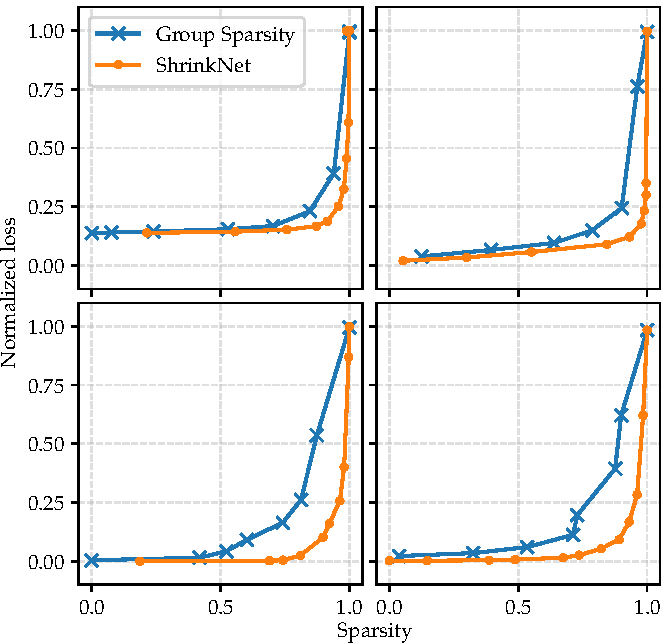
\includegraphics[height=0.97\columnwidth]{regressions}
\vspace*{-5mm}
\caption{\label{sparsity_accuracy}Loss/Sparsity trade off comparison between Group Sparsity and Shrinknet on linear and logistic regression. From top to bottom and left to right we show the results for \texttt{scm1d}, \texttt{oes97}, \texttt{gina\_prior2} and \texttt{gsadd}.}

\end{center}
\vspace*{-4mm}
\end{figure}

\subsection{Neuron Removal strategies}

In our previous experiment, we showed that the ShrinkNet loss was
reasonable in practice, we are now interested in the impact on
early pruning. The two most important questions to answer are:
What are the impact on convergence speed (i.e. the number of iterations) ?
and: What is the difference in loss with and without early pruning ?

\subsection{Convergence and training dynamics of Neural networks}

\subsection{Hyper-optimization of ShrinkNets}

\subsection{Performance}

\section{Related Work}

\section{Future Work}

\section{Conclusion}

\appendix
\section{Appendix}
\subsection{Proofs}
Unless specified, all the proofs consider the Multi-Target linear regression problem
\begin{proposition}
\label{gps_equivalence}
  $\forall (n, p) \in \mathbb{N}_+^2, \bm{y} \in \mathbb{R}^{n}, \bm{x} \in \mathbb{R}^{p} \lambda \in \mathbb{R}$
  
  \begin{align*}
    & \min_{\bf{A}} \norm{\bf{y} - \bf{A}\bf{x}}_2^2 + \lambda \sum_{j=1}^p \norm{\left(A^T\right)_j}_2 \\
     = &\min_{\bf{A'}, \bm{\beta}} \norm{\bf{y} - \bf{A'}\diag{\bm{\beta}}\bf{x}}_2^2 + \lambda \norm{\bm{\beta}}_1 \\
     & \text{s.t.} \forall j \in \intint{1, p}, \norm{\left(A'^T\right)_j}_2^2 = 1
  \end{align*}
\end{proposition}

\begin{proof}
  In order to prove this statement we will show that for any solution $\bm{A}$ in the first problem, there exists a solution in the second with the exact same value, and vice-versa.
We now assume we have a potential solution $\bm{A}$ for the first problem and we define $\bm{\beta}$ such that $\bm{\beta}_j = \norm{\left(\bm{A}^T\right)_j}_2^2$, and $\bm{A}' = \bm{A}\left(\diag{\bm{\beta}}\right)^{-1}$. It is easy to see that the constraint on $\bm{A}'$ is statisfied by construction. Now:
  \begin{align*}
    & \norm{\bf{y} - \bf{A}\bf{x}}_2^2 + \lambda \sum_{j=1}^p \norm{\left(A^T\right)_j}_2 \\
    = &\norm{\bf{y} - \bf{A'}\diag{\bm{\beta}}\bf{x}}_2^2 + \lambda \sum_{j=1}^p \norm{\left(A'^T\right)_j\beta_j}_2 \\
    = &\norm{\bf{y} - \bf{A'}\diag{\bm{\beta}}\bf{x}}_2^2 + \lambda \sum_{j=1}^p \abs{\beta_j} \cdot 1\\
    = &\norm{\bf{y} - \bf{A'}\diag{\bm{\beta}}\bf{x}}_2^2 + \lambda \norm{\bm{\beta}}_1
  \end{align*}
  Assuming we take an $\bm{A}'$ that satisfy the constraint and a $\bm{\beta}$, we can define $\bm{A} = \bm{A'}\diag{\bm{\beta}}$. We can apply the same operations in reverse order and obtain an instance of the first problem with the same value. We can now see that the two problems must have the same minimum otherwise we would be able to construct a solution to the other with exact same value.
\end{proof}

\begin{proposition}
\label{unconstrained_non_convex}
\begin{equation*}
     \norm{\bf{y} - \bf{A}\diag{\bm{\beta}}\bf{x}}_2^2
\end{equation*}
is not convex in $\bm{A}$ and $\bm{\beta}$.
\begin{proof}
  To prove this we will take the simplest instance of the problem: with only scalars. We have $f(a, \beta) = \left(y - a\beta x\right)^2$. For simplicty let's take $y = $ and $x > 0$. If we take two candidates $s_1 = (0, 2)$ and $s_2 = (2, 0)$, we have $f(s_1) = f(s_2) = 0$. However $f(\frac{2}{2}, \frac{2}{2}) = x > \frac{1}{2} f(0, 2) + \frac{1}{2}f(2, 0)$, which break the convexity property. Since we showed that a particular case of the problem is non-convex then necessarly the general cannot be convex.
\end{proof}
\end{proposition}

\begin{proposition}
\label{unconstrained_shrinknet_no_min}
\begin{equation*}
     \min_{\bf{A}, \bm{\beta}} \norm{\bf{y} - \bf{A}\diag{\bm{\beta}}\bf{x}}_2^2 + \lambda \norm{\bm{\beta}}_1
\end{equation*}
has no solution if $\lambda > 0$.
\end{proposition}
\begin{proof}
  Let's assume this problem has a minimum $\bm{A}^*, \bm{\beta}^*$. Let's consider $2\bm{A}^*, \frac{1}{2}\bm{\beta}^*$. Trivially the first component of the sum is identical for the two solutions, however $\lambda\norm{\frac{1}{2}\bm{\beta}} < \lambda\norm{\bm{\beta}}$. Therefore $\bm{A}^*, \bm{\beta}^*$ cannot be the minimum. We conclude that this problem has no solution.
\end{proof}
\begin{proposition}
  \label{shrinknet_regularized_minimum}
For this proposition we will not restrict ourselves to single layer but the composition of an an arbitrary large ($n$) layers as defined individually as $f_{\bm{A}_i, \bm{\beta}_i, \bm{b}_i}(x) = a(\bm{A_i}\diag{\bm{\beta_i}}\bm{x} + \bm{b_i})$. The entire network follows as: $N(\bm{x}) = \left(\bigcirc_{i=1}^n f_{\bm{A_i}, \bm{\beta_i}, \bm{b_i}}\right)(\bm{x})$. For $\lambda > 0$, $\lambda_2 > 0$ and $p > 0$ we have:
  \begin{equation*}
    \min \norm{\bm{y} - N(\bm{x})}_2^2 + \Omega_{\lambda, \lambda_2, p}^{rs}
  \end{equation*}
  has at least $2^k$ global minimum where $k = \sum_{i=1}^n \#\bm{\beta_i}$
\end{proposition}

\begin{proof}
First let's prove that there is at least one minimum to this problem. The two components of the expression are always positive so we know that this problem is bounded by below by $0$. Let's assume this function does not have a minimum. Then there is a sequence of parameters $(S_n)_{n>0}$ such that the function evaluated at that point convereges to the infimum of the problem. Since the function is defined everywhere does not have a minimum then this sequence must diverge. Since the entire sequence deverge the there is at least one individual parameter that diverges. First case, the parameter is a component $k$ of some $\bm{\beta_i}$ for some $i$. Necessarly $\norm{\bm{\beta_i}}_1$ diverge towards $+ \infty$, which is incompatible with the fact that $(S_n)$ converges to the infimum. We can have the exact same argument if the diverging parameter is in $\bm{A_i}$ or $\bm{b_i}$ because $p > 0$. Since there is always a contradiction then our assumption that the function has no global minimum must be false. Therefore, this problem has at least one global minimum.

\par Let's consider one optimal solution of the problem. For each component $k$ of $\bm{\beta_i}$ for some $i$. Negating it and negating the $k^{th}$ column of $\bm{A_i}$ does not change the the first part of the objetive because the two factors cancel each other. The two norms do not change either because by definition the norm is independant of the sign. As a result these two sets of parameter have the same value and are both global minimum. It is easy to see that going from this global minimum we can decide to negate or not each element in each $\bm{\beta_i}$. We have a binary choice for each parameter, there are $k = \sum_{i=1}^n \#\bm{\beta_i}$ parameters, so we have at least $2^k$ global minima.

\end{proof}
\subsection{Experiment details}
\subsubsection{Multi-Target Linear and Logistic regressions}
\label{linear_datasets}
\subsubsection{Neuron Removal strategies}
\subsubsection{Convergence and Training Dynamics of Neural networks}
\subsubsection{Hyper-optimization of ShrinkNets}
\subsubsection{Performance}


% In the unusual situation where you want a paper to appear in the
% references without citing it in the main text, use \nocite
\nocite{OpenML2013}

\bibliography{custom}
\bibliographystyle{icml2018}



\end{document}
